\section{介绍}

金融市场基础设施(FMI)是由多个彼此独立的参与机构形成的多边系统,这些设施有助于支付、证券、衍生品合约等货币和其它金融交易的清算、结算和记录。是金融运行的的基础。
它是金融经济系统高效、安全运行的重要保证。对于畅通货币政策传导机制、加速社会资金周转、优化社会资源配置、维护金融稳定并促进经济增长有重要意义。

现代金融市场基础设施虽然在不同国家有不同的具体组织形式,但一般包含以下五种基本职能及对应的支撑机构:

\begin{itemize}
    \item [\dag] \textbf{支付功能}:支付系统(Payment System) 提供资金转账服务。
    \item [\dag] \textbf{存管功能}:中央证券存管(Central Securities Depository ,CSD) 提供证券集中发登记、托管、赎回等服务。
    \item [\dag] \textbf{清算功能}:中央对手方(Central Counter Party ,CCP) 作为一种清算机制,清算机构自身介入已经达成的交易,成为卖方的买方和买方的卖方,确保已达成交易正常履约,是防范金融市场系统性风险的重要手段。
    \item [\dag] \textbf{结算功能}:证券结算系统(Securities Settlement system,SSS) 提供证券过户和结算服务(如典型的券款对付DvP)。
    \item [\dag] \textbf{报告功能}:交易数据库(Trade Repository ,TR)是为增强市场透明性而集中收集、保存并向监管和公众披露各类交易数据的机构,是金融危机后为加强场外衍生品市场监管而新出现的FMI类型。
\end{itemize}

现代金融市场基础设施为全球金融市场交易提供了一个相对稳定、可靠的基础和环境。但仍然存在一定局限: 
\begin{enumerate}
    \item 今天的金融市场由众多不同层级的参与者组成,并形成了一个复杂的网络,其业务流程和相关技术系统也非常复杂,同时许多手工处理步骤依然存在。
    \item 每一个参与者需要保存和维护自己独立、专有的数据库,每一交易数据的变化需要通知利益相关者并需要在不同系统之间进行对账或保持一致。
    \item 交易以及清算,结算和抵押品管理等系统,在不同历史时期为了不同的需要而建立,没有广泛接受的标准,系统之间缺乏互操作性。
\end{enumerate}
金融市场基础设施的这些局限,不仅使结算周期变长、增加后台处理成本,也增加了整个金融市场的风险。

2008年金融危机爆发以来,国际社会对引起危机的根源进行了深刻反思,结论之一就是要加强安全、高效、透明、规范的金融市场基础设施建设。
分布式账本作为一种新的账本管理技术,非常有潜力改善现有金融市场基础设施的局限性。
它与传统中心化、层级化的交易处理和记账方式截然不同。分布式账本的去中心化特性,可以用来消除一些金融市场中间环节、实现点对点直接交易,从而简化业务流程,缩短交易周期,有效降低风险、提高效率、节约成本。

Libra 的使命之一是基于分布式账本技术,建立一套通用的、无国界的、为数十亿人服务的金融市场基础设施,创造一个更加普惠的金融体系。
金融是一个强监管的行业,金融市场基础设施在金融的监管体系中扮演了关键的角色,它们为金融市场指定了统一的流程、规则;
而且监管层可以通过它们监管整个金融系统。
下图是美国金融监管架构图\footnote{源自芝加哥联邦储备银行:\url{https://www.chicagofed.org/markets/view-lasalle-street/us-reg-authority}},从中可以看到基础设施在金融监管方面的重要作用。

\begin{figure}[h!]
    \centering
    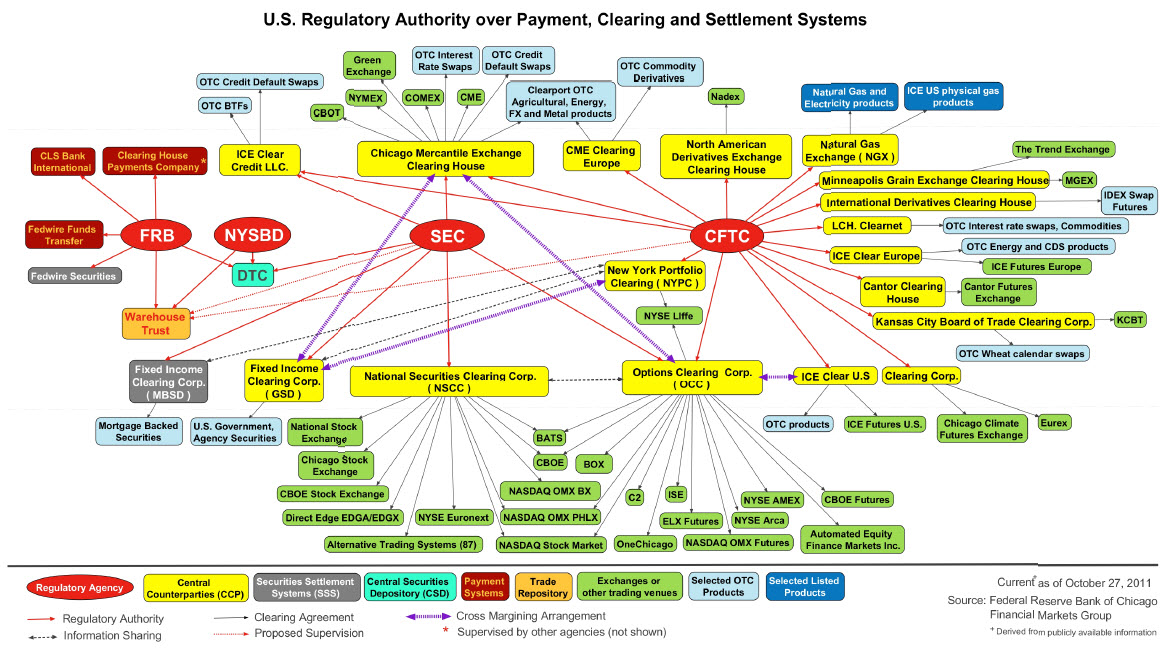
\includegraphics[width=12cm, keepaspectratio]{images/regulatory-over-PCS.jpg}
    \caption{美国联邦金融监管架构}
    \label{fig:USAReg}
\end{figure}

%基于上述这些基础设施服务机构,其它金融机构,如交易场所(交易所或场外市场)、证券发行方、托管银行、买方/卖方、经纪商、清算会员、结算代理行等,面向用户展开各种金融服务。它们共同形成了一个多层级的、互相协作、互相制约的复杂网络。

我们认识到,Libra 必须要满足金融监管与合规的需求,才能成为可大规模应用的金融市场基础设施。在7月16与17日举行的 Libra 听证会上,美国参众两院也提出了一些列关于金融监管与合规的要求。作为回应,此白皮书将介绍 Libra 网络在了解客户(KYC), 反洗钱(AML)、反恐怖主义融资(CFT)等方面的解决方案。

本文的结构如下:
\begin{itemize}
    \item[] 第2章:介绍分布式账本技术(DLT)与金融市场基础设施原则(PFMI)的关系。
    \item[] 第3章:介绍账本管理的三元悖论,解释分布式账本固有的抗审查性。
    \item[] 第4章:介绍加拿大央行、欧洲央行、日本央行、新加坡金融管理局的相关工作和结论。
    \item[] 第5章:介绍记账权与审核权的分离,在Libra生态中,金融机构负责合规,矿工负责记账。
    \item[] 第6章:介绍与合规相关的账本数据结构,支持与链下的身份管理系统集成。
    \item[] 第7章:介绍分层的账户体系结构与准入机制。
    \item[] 第8章:介绍交易前置的合规验证协议,与链下的反洗钱等合规系统集成。
\end{itemize}

%\begin{figure}[h!]
%    \centering
%    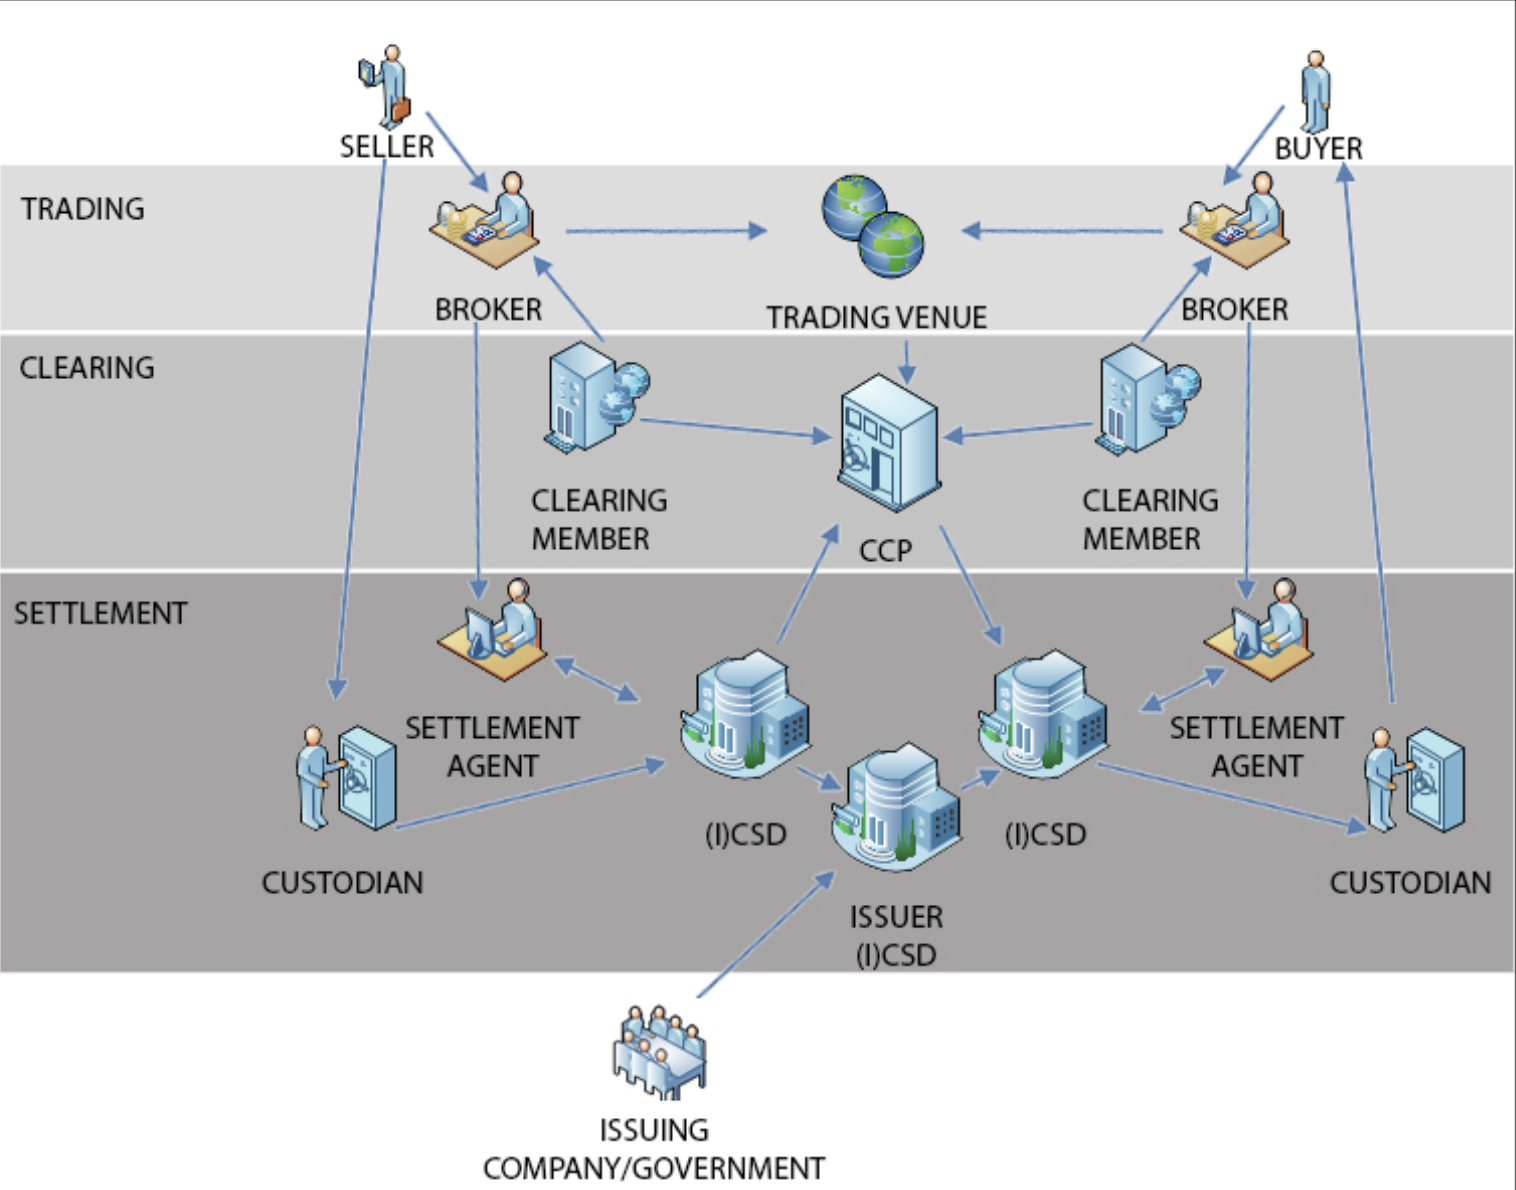
\includegraphics[width=8cm, keepaspectratio]{images/Security-Arch.png}
%    \caption{证券金融基础设施}
%    \label{fig:security}
%\end{figure}


